% Created 2024-11-25 man 22:01
% Intended LaTeX compiler: xelatex
\documentclass[a4paper, 12pt]{article}
\usepackage{graphicx}
\usepackage{longtable}
\usepackage{wrapfig}
\usepackage{rotating}
\usepackage[normalem]{ulem}
\usepackage{amsmath}
\usepackage{amssymb}
\usepackage{capt-of}
\usepackage{hyperref}
\usepackage[danish]{babel}
\usepackage[margin=3.0cm]{geometry}
\usepackage{hyperref}
\hypersetup{colorlinks, linkcolor=black, urlcolor=blue}
\setlength{\parindent}{0em}
\parskip 1.5ex
\author{Jacob Debel}
\date{Fysik B}
\title{Mekanik\\\medskip
\large Ballistisk bevægelse (Det skrå kast)}
\hypersetup{
 pdfauthor={Jacob Debel},
 pdftitle={Mekanik},
 pdfkeywords={},
 pdfsubject={},
 pdfcreator={Emacs 29.4 (Org mode 9.6.15)}, 
 pdflang={Danish}}
\begin{document}

\maketitle


\section*{Opgave 1}
\label{sec:org375fe2c}

En fodbold sparkes afsted med en starthastighed på 16 m/s og en vinkel på 20 grader med vandret.

\begin{enumerate}
\item Indtegn bolden og startbetingelserne i et selvvalgt koordinatsystem.
\item Bestem den tid det tager for bolden at nå sit toppunkt.
\item Hvad er koordinaterne til toppunktet i jeres selvvalgte koordinatsystem?
\item Bestem den maksimale længde(kastevidden).
\item (Ekstra) Hvor lang skal afstanden være for at bolden netop rammer overlæggeren på et 11-mandsmål, hvis det overhovedet er muligt? (Højden er 2.44 m)
\end{enumerate}

\section*{Opgave 2}
\label{sec:org4987828}

En kugle triller med konstant hastighed hen over en vandret bordplade i højden 85 cm over gulvet. Kuglen lander 40 cm fra bordkantens lodrette projektion på gulvet.

\begin{enumerate}
\item Tegn en skitse over situationen.
\item Hvor lang er faldtiden?
\item Hvad var kuglens hastighed umiddelbart før den forlod bordpladen?
\item Hvad er kuglens fart umiddelbart før den rammer gulvet?
\end{enumerate}

\newpage

\section*{Opgave 3}
\label{sec:orgdadba21}

En golfspiller står ved et “dogleg” par 4-hul.

\begin{center}
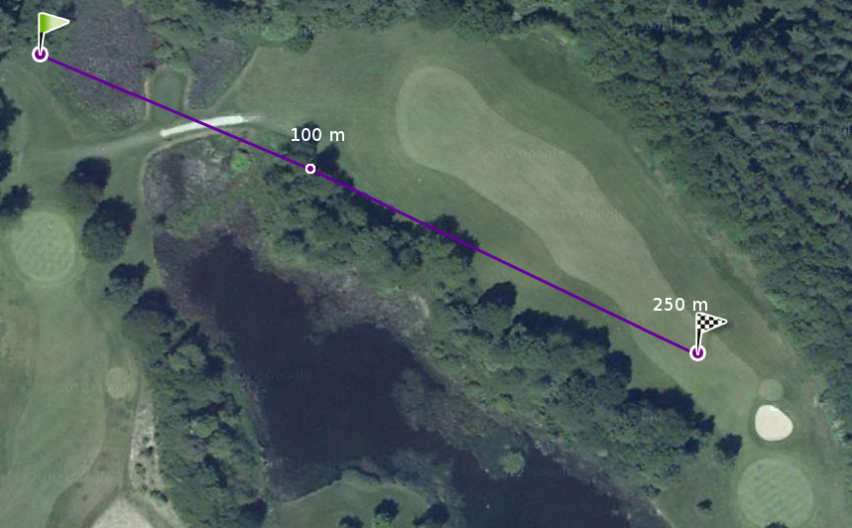
\includegraphics[width=0.7\linewidth]{img/golf.png}
\end{center}

Golfspilleren ved at han kan slå 250 m med sin driver, som har en vinkel på 11 grader.

\begin{enumerate}
\item Vis, for sådan et slag, at boldens tid i luften er 3.14 sek og boldens starthastighed er 80.95 m/s. (To ligninger med to ubekendte.)
\item Kan spilleren, med et sådant slag, tage en genvej hen over træerne eller skal han spille den safe? Træerne 100 m foran ham er 12 m høje.
\end{enumerate}


\section*{Opgave 4}
\label{sec:org416a248}

“Ghost Rider” vil forsøge et spring som vist på figuren.
\begin{center}

\includegraphics[height=0.23\textwidth]{img/2019-10-30_10-35-14_maxresdefault.jpg}
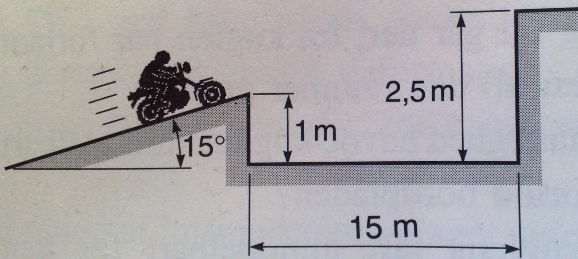
\includegraphics[height=0.23\textwidth]{img/ghost_rider.png}
\end{center}

Rampen hælder 15 grader med vandret, og starthastigheden er 100 km/h.

\begin{enumerate}
\item Hvor højt passerer han over kanten på plateauet?
\item Hvor lang tid er han i luften inden han lander på plateauet?
\item Hvad er den minimale fart Ghost Rider kan have for at springet fuldføres?
\end{enumerate}

\section*{Opgave 5 (Ekstra)}
\label{sec:org44f8702}

\begin{enumerate}
\item Find, via de generelle formler for det skrå kast, et udtryk for nedslagstiden som funktion af “affyringsvinklen”.
\item Bestem den affyringsvinkel som giver den maksimale længde.
\end{enumerate}
\end{document}
